
\chapter{Valuación de opciones usando CAPM}\label{ValuacionMedianteCAPM}

\section{Relación matemática entre CAPM y B\&S}

Estos dos modelos parten de diferentes supuestos como se explicó los capítulos anteriores. CAPM parte de un equilibrio de mercado para derivar la \textit{Capital Market Line} y hallar el portafolio óptimo. Por el otro lado, el modelo de Black-Scholes utiliza un supuesto de no-arbitraje para valuar opciones. Si bien ambos supuestos son notablemente diferentes, no son contrapuestos en un mercado eficiente. Como se verá a continuación, ambos modelos conllevan a los mismos resultados \cite{kishimoto}.

Partiendo de la ecuación resultante del lema de \textit{Ito} \eqref{ito-ftaylor} y de la definición del movimiento browniano geométrico que sigue el precio de una acción \eqref{brownianmotion}:

\begin{align}
	df &= \frac{\partial f}{\partial S} dS + 
		\frac{\partial f}{\partial t} dt + 
		\frac{1}{2} \frac{\partial^2 f}{\partial S^2} (dS)^2 \tag{\ref{ito-ftaylor}} \\
	dS &= \mu S dt + \sigma S dW \tag{\ref{brownianmotion}}
\end{align}

Luego, reemplazando \eqref{brownianmotion} en \eqref{ito-ftaylor}:

\begin{align}
	df = \frac{\partial f}{\partial t} dt +
		\frac{\partial f}{\partial S} (\mu S dt + \sigma S dW) +
		\frac{1}{2} \frac{\partial^2 f}{\partial S^2} \left[ \mu^2 S^2 dt^2 + 2 \mu S^2 \sigma dt dW + \sigma^2 S^2 dW^2 \right]
		\label{capmbs1}
\end{align}

Debido a que tanto $dt^2$ como $dt dW$ son de orden mayor a uno - recordar que $dW = Z \sqrt{dt}$ -, se pueden considerar a ambos términos despreciables. Por el otro lado, el término $dW^2 = Z^2 dt$ puede ser analizado de la siguiente forma: $E[Z^2] = E[(Z - E[Z])^2]$, pero debido a que $Z$ es una normal con media cero, la esperanza de $Z$ será a su vez cero. Por lo tanto $dW^2$ es igual a $dt$, ya que $E[Z^2]$ se corresponde con la varianza de $Z$, la cual es igual a 1 por definición.

Si ahora se introduce \eqref{brownianmotion} en \eqref{capmbs1} y se divide a todo por $f$, se llega a que:

\begin{align}
	\frac{df}{f} = \frac{S}{f} \frac{\partial f}{\partial S} \frac{dS}{S} +
		\frac{1}{f} \left( \frac{\partial f}{\partial t} +
			\frac{1}{2} \frac{\partial^2 f}{\partial S^2} \mu^2 S^2
		\right) dt \label{capmbs3}
\end{align}

Las expresiones $df/f$ y $dS/S$ corresponden con los rendimientos del derivado y del subyacente respectivamente, por lo que se puede calcular la covarianza en ambos lados de la ecuación \eqref{capmbs3} con los rendimientos del mercado ($r_m$). De esta forma se obtiene:

\begin{align}
	Cov(\frac{df}{f}; r_m) &= \frac{S}{f} \frac{\partial f}{\partial S} Cov(\frac{dS}{S}; r_m) \\
	\beta_f &= \frac{S}{f} \frac{\partial f}{\partial S} \beta_S \label{relacionbetas}
\end{align}

La ecuación \eqref{relacionbetas} presenta la relación entre los \textit{betas} de la opción y del subyacente, las cuales se analizarán más adelante en este capítulo.

Según CAPM el retorno esperado de una opción estará dado por \cite{frouah-formula}:

\begin{equation}
	E\left[ \frac{df}{f} \right] = r dt + \beta_f (E[r_m] - r) dt \label{opcionporcapm}
\end{equation}

Multiplicando ambos términos por $f$ y reemplazando $\beta_f$ por la equivalencia encontrada en \eqref{relacionbetas}, se obtiene:

\begin{equation}
	E[df] = r f dt + \frac{\partial f}{\partial S} S \beta_S (E[r_m] - r) dt
\end{equation}

Nuevamente tomando la ecuación \eqref{capmbs3} multiplicada por $f$, y reemplazando $dS$ por la relación que CAPM establece, se llega a que:

\begin{equation}
	E[df] = \frac{\partial f}{\partial S} r S dt + 
		\frac{\partial f}{\partial S} \beta_S S (E[r_m] - r) dt +
		( \frac{\partial f}{\partial t} + \frac{1}{2} \sigma^2 S^2 \frac{\partial^2 f}{\partial S^2}) dt
\end{equation}

Lo cual se puede igualar a la ecuación \eqref{opcionporcapm} y reorganizar para llegar a la ecuación de derivadas parciales de Black-Scholes \cite{frouah-formula}:

\begin{equation}
	r f = \frac{\partial f}{\partial t} + r S \frac{\partial f}{\partial S} +
		\frac{1}{2} \sigma^2 S^2 \frac{\partial^2 f}{\partial S^2}
\end{equation}

La principal característica de esta última formula derivada es que es dependiente del modelo de CAPM, por lo cual se establece una relación entre estos dos modelos. Diversos autores presentan esta relación, a continuación se desarrolla la valuación de una opción utilizando el modelo de CAPM para mostrar sus resultados.


\section{El cálculo mediante CAPM}

Como se explicó anteriormente el modelo desarrollado por Sharp plantea un equilibrio de mercado en términos de rentabilidad y riesgo. Es por esto que las opciones sobre acciones que cotizan en el mercado deben lógicamente cumplir con este equilibrio. Si esto no ocurriese, los participantes del mercado deberían incluir o excluir estos activos de su portafolio para maximizar su utilidad, o la pendiente de la \textit{CML} en términos de CAPM. 

A continuación se realizan dos derivaciones que permiten obtener el valor de el \textit{beta} de la opción en tiempo discreto y luego el precio de la opción utilizando CAPM.

\subsection{Obteniendo el \textit{beta} por réplica}

Se puede pensar a una opción como un portafolio que incluya a la acción subyacente y un bono como se mostró en el capítulo anterior. Por esta razón, en ausencia de oportunidades de arbitraje, tanto el portafolio replicante como la opción deben valer lo mismo. Para realizar un portafolio que tenga el mismo \textit{payoff} que la opción se debe tener $ \Delta $ unidades del subyacente y una cantidad $B$ en un bono como se mostró en las ecuaciones \eqref{portReplDelta} y \eqref{portReplB}.

A los argumentos de equilibrio de mercado desarrollado por William Sharp y del de no arbitraje, se le suma el argumento de la ley de precio único (que está estrechamente ligada al argumento de no-arbitraje). Este último se basa en el hecho de que, al existir la posibilidad de replicar la opción utilizando un acción y un bono, tanto el portafolio replicante como la opción deberían tener el mismo precio.

Nuevamente, el portafolio replicante está dado por $\Delta$ \eqref{portReplDelta} y $B$ \eqref{portReplB}. A su vez, se sabe que el \textit{beta} de un portafolio se calcula como el promedio ponderado de los activos que lo componen \cite[p.135]{hull}, por lo que el \textit{beta} del portafolio replicante estará dado por:

\begin{equation}
	\beta_f = \frac{\Delta S}{\Delta S + B} \beta_S + \frac{B}{\Delta S + B} \beta_B \label{prombetarepl}
\end{equation}

Debido a que el \textit{beta} de la deuda puede ser considerada igual cero, se sabe que el \textit{beta} de la opción está dado por $ \beta_f = \frac{\Delta S}{\Delta S + B} \beta_S $. La ecuación \eqref{relacionbetas} presenta otra fórmula válida para el cálculo del \textit{beta} de las opciones, sin embargo \eqref{prombetarepl} es más sencilla de calcular ya que no depende del precio actual de la opción.

Dado que se sabe el valor del \textit{beta} de la opción, se puede calcular el retorno esperado mediante CAPM, de forma que:

\begin{equation}
	E[r_f] = r + \frac{\Delta S}{\Delta S + B} \beta_S (E[r_m] - r) \label{rcopcion}
\end{equation}

De esta forma se sabe que el rendimiento estará dado por \eqref{rcopcion}, el cual tiene que coincidir con el rendimiento esperado en el árbol binomial\footnote{Un desarrollo similar para el caso de valuación neutral al riesgo puede verse en Hull (2009b).\nocite{hulleng}}.
Por lo tanto, la expresión \eqref{matchingprob} muestra el valor $S_0$ multiplicado por el promedio ponderado de los posibles retornos totales \cite{appliedderiv}:

\begin{equation}
	p S_0 \mu + (1-p) S_0 d = S_0 (1 + r_S) \label{matchingprob}
\end{equation}

Siendo $p$ la probabilidad que hace que $r_S$ sea el rendimiento dado por CAPM. Sin embargo, al mismo tiempo es necesario que la volatilidad de los rendimientos del árbol coincida con la de la acción \cite{hulleng}. Es por eso que al mismo tiempo debe cumplirse la condición de que:

\begin{align}
	p \mu^2 + (1-p) d^2 - [p \mu  + (1-p) d]^2 = \sigma^2 \Delta t \label{matchvolat}
\end{align}

Donde $\sigma^2 \Delta t$ es la volatilidad del subyacente\footnote{Véase Hull (2009b), capítulo 13.}.

Las constante $p$, $d$ y $\mu$ deben satisfacer las ecuaciones \eqref{matchingprob} y \eqref{matchvolat} de forma que el rendimiento y la volatilidad esperada sean las adecuadas para el portafolio replicante. Por ejemplo, Ross, Cox y Rubinstein resuelven el problema en tiempo continuo (rendimiento esperado $e^{r \Delta t}$) definiendo $\mu = e^{\sigma \sqrt{\Delta t}}$, $d=1/\mu$ y $p=\frac{e^{\sigma \Delta t}-d}{\mu-d}$. Dado que son dos ecuación y tres incógnitas, existen infinitas soluciones al problema. Para el caso en que el árbol binomial tiene la rentabilidad esperada por CAPM, se puede despejar la ecuación \eqref{matchingprob} de forma que:

\begin{align}
	p = \frac{1 + r_s \Delta t - d}{\mu-d} \label{probarbolcapm}
\end{align}

Y se mantiene $\mu = e^{\sigma \sqrt{\Delta t}}$ y $d=1/\mu$, de forma que las dos ecuaciones se satisfacen y tanto la volatilidad como el rendimiento esperado del árbol son iguales a los esperados del subyacente.

Por último, el valor de la opción estará dado por el \textit{payoff} futuro descontado a la tasa de retorno esperada por el modelo de Sharp:

\begin{equation}
	f = \frac{1}{1 + r_f \Delta t} [p f_\mu + (1-p) f_d] \label{discountPayoffs}
\end{equation}


\subsection{Obteniendo el \textit{beta} por definición}

Por el otro lado, también se puede partir de la ecuación \eqref{relacionbetas} que se derivo anteriormente. La expresión $\partial f / \partial S$ en tiempo discreto para el árbol binomial está dado por $\Delta$ \cite{appliedderiv}, por lo que:

\begin{align}
	\Delta &= \frac{ f_\mu - f_d }{ S \mu - S d }\\
	\beta_f &= \Delta \frac{S}{f} \beta_S \label{relacionbetascomoderiv}
\end{align}

Sin embargo, la ecuación \eqref{relacionbetascomoderiv} muestra que $\beta_f$ es dependiente del precio del derivado $f$. Siguiendo el procedimiento realizado en la sección anterior, calcular el precio de este directamente no es posible ya que para calcular la tasa de descuento $r_f$ es necesario obtener el \textit{beta} de la opción; y para obtener esta última es necesario conocer el precio de la opción. De esta forma, el problema se vuelve recursivo.

Se puede plantear una sistema de ecuaciones ya que existen solo dos incógnitas $f$ y $\beta_f$, de la siguiente manera:

\begin{align}
	\beta_f &= \beta_S \frac{f_\mu - f_d}{S(\mu-d)} \frac{S}{f} \label{betapordef1} \\
	\overline{r_f} &= r + \beta_f (\overline{r_M} - r) \label{betapordef2} \\
	f &= \frac{1}{1+r_f \Delta t} \left[p f_\mu + (1-p) f_d \right] \label{betapordef3}
\end{align}

Donde los parámetros $p$, $\mu$ y $d$ no dependen del valor de $f$. De esta forma se puede reemplazar \eqref{betapordef1} en la ecuación \eqref{betapordef2} y a su vez esta última en la ecuación \eqref{betapordef3}. Con matemática simple se puede despejar el valor de la opción de forma de obtener una fórmula no dependiente de si misma:

\begin{align}
	f &= \frac{1}{1+r \Delta t} \left[p f_\mu + (1-p) f_d - 
		\beta_S \frac{f_\mu - f_d}{\mu-d} (\overline{r_M} - r) \Delta t \right] \label{opciondespejadodirect}
\end{align}

Evaluando la ecuación \eqref{opciondespejadodirect} se puede llegar al mismo resultado que con el mecanismo mencionado anteriormente. En este caso se partió de la definición matemática de \textit{beta} para el modelo discreto \cite{appliedderiv} en vez de hallar un valor partiendo del portafolio replicante. 

\subsection{Portafolio replicante}

A modo de ejemplo, supongamos un subyacente con precio inicial $S_0 = 100$, desvío estándar anual esperado $\Sigma = 0.2$, \textit{Strike Price} $X=100$, la tasa de interés libre de riesgo es $r=3\%$, el \textit{beta} de la acción es igual a uno, prima de riesgo de mercado igual a 6\% y $\Delta t = 0.05$. Primero se debe calcular $\mu$ y $d$ para el árbol binomial, de forma que:

\begin{align}
	\mu &= e^{\sigma \sqrt{\Delta t}} = 1.0457\\
	d &= 1/\mu = 0.9563
\end{align}

Por lo que $S \mu = 104.57$ y $S d = 95.63$, el árbol de un paso sería como el de la figura \ref{fig:arbolunpasocapm}.

\begin{figure}[H]
\centering
\includegraphics[width=153px]{Images/EjemploArbol1Paso.jpg}
\caption{Árbol de un paso}
\label{fig:arbolunpasocapm}
\end{figure}

Si la opción es un \textit{call}, a su vez se sabe que el \textit{payoff} estará dado por $(S_T - X)^+$, y en este caso el precio de la opción al vencimiento será $c_\mu = 4.57$ o $c_d = 0$. Como la opción es replicable por el subyacente más un prestamo, se puede hallar las proporciones que replican el derivado de esta forma:

\begin{align}
	c &= \Delta S + B\\
	\Delta &= \frac{c_\mu - c_d}{S(\mu - d)} = 0.51\\
	B &= \frac{\mu C_d - d c_\mu}{(\mu-d)e^{r \Delta t}} = -48.81
\end{align}

Esto indica que la opción puede ser replicada comprando 0.51 unidades del subyacente y obteniendo un préstamo de \$48.81, lo que haría que la compra quede en su mayoría financiada por el préstamo.

El $\beta$ de un portafolio es el promedio ponderado de los \textit{betas} de los activos que lo componen, por lo que el \textit{beta} de la opción lógicamente será un promedio entre el \textit{beta} de la acción y el del préstamo. Este último al ser constante y no estar correlacionado con el mercado tiene $\beta = 0$. Entonces:

\begin{align}
	\beta_c &= \frac{\Delta S}{\Delta S + B} \beta_S + \frac{B}{\Delta S + B} \beta_B \\
	\beta_c &= \frac{\Delta S}{\Delta S + B} \beta_S \label{betaopcionporrepl} \\
	\beta_c &= 23.29
\end{align}

Y la rentabilidad esperada de la opción acorde al modelo de CAPM, será:

\begin{align}
	r_c &= r + \beta_c (E[r_m] - r) = 1.427
\end{align}

Por último, sabiendo que la rentabilidad esperada de la acción está dada por $r_s = r + \beta_S (E[r_m] - r) = 9\%$, se puede calcular la probabilidad $p$ y el precio de la opción en el momento cero:

\begin{align}
	p &= \frac{1 + r_s \Delta t - d}{\mu - d} = 0.5391\\
	c &= \frac{1}{1+r_c \Delta t} \left[ p c_\mu + (1-p) c_d \right] = 2.30
\end{align}


Entonces el precio de la opción en el momento cero será 2.30. Claro que el árbol en este caso es de un solo paso, lo cual lleva a errores significativos. Para que la precisión del mismo sea buena, el procedimiento debe repetirse en un árbol con un gran número de pasos.

\section{Arboles de grado \textit{n}}

En el caso de árboles con una mayor cantidad de pasos, el procedimiento es similar al realizado anteriormente. A diferencia de la resolución utilizada en el método de Ross et al (1979)\nocite{rosscoxrubinstein}, parámetros adicionales tales como la $\beta$ y la tasa de descuento deben ser recalculados en cada momento del árbol.

Primero, deben obtenerse los precios del subyacente para cada nodo del árbol, esto se hace partiendo desde el primer nodo y multiplicándolo por $\mu$ en caso de que el precio suba, o por $d$ en caso de que baje. Una vez obtenidos los precios finales, se puede calcular el precio al final del árbol en cada nodo debido a que el \textit{payoff} es conocido e igual a $\mbox{max}(S_T - X;0)$ para el caso de las opciones de compra.

Luego, debe recorrerse el árbol en orden inverso, es decir desde el último paso hasta el primero ya que los nodos del paso $i-1$ dependen de los del paso $i$. La fórmula para calcular el precio de la opción en cada nodo está dada por \eqref{discountPayoffs} como se mostró anteriormente. Para el caso del \textit{call} quedaría:

\begin{equation}
	c = \frac{1}{1 + r_c \Delta t} [p c_\mu + (1-p) c_d] \tag{\ref{discountPayoffs}}
\end{equation}

Donde $r_c$ es el retorno esperado para la opción y $p$ la probabilidad de que ocurra una suba en el precio. En el caso de Ross et al (1979)\nocite{rosscoxrubinstein} la tasa de descuento es la tasa libre de riesgo, ya que ellos realizan una valuación en un mundo neutral al riesgo, lo cual es válido ya que el portafolio se valúa por réplica. Sin embargo, en este caso la tasa de descuento es dependiente de la rentabilidad real esperada de la opción \cite{optionsmarkets}, la cual puede ser calculada mediante la técnica de no arbitraje como se vio anteriormente. Como consecuencia, para cada nodo es necesario realizar el cálculo de la tasa de descuento como se verá a continuación, lo cual agrega la necesidad de computar datos adicionales.

La probabilidad $p$ está dada por la ecuación \eqref{probarbolcapm} de acuerdo a la volatilidad y la rentabilidad del subyacente.

\begin{equation}
	p = \frac{1 + r_S \Delta t - d}{\mu - d} \tag{\ref{probarbolcapm}}
\end{equation}

Donde $r_S$ es la rentabilidad de la acción subyacente, que puede ser calculada utilizando CAPM como se ve en la ecuación \eqref{capm}. $\mu$ y $d$ son parámetros que se calculan de igual forma que en la solución de Ross-Cox-Ingersoll. 

Finalmente, la rentabilidad esperada de la opción según el modelo de William Sharp estará dada por la ecuación \eqref{rcopcion}:

\begin{equation}
	E[r_c] = r + \frac{\Delta S}{\Delta S + B} \beta_S (E[r_m] - r) \tag{\ref{rcopcion}}
\end{equation}
	
Este mismo proceso se debe repetir en todos los nodos del árbol desde el último paso hacia el primero. Para obtener un valor exactamente igual al que se puede obtener por el método de Black-Scholes, que es en tiempo continuo, la cantidad de pasos $n$ debe tender a infinito. Sin embargo, todos los árbol binomiales son funciones exponenciales y agregar precisión es costoso de computar. Más adelante en este capítulo se analiza la precisión de estos arboles en función de la cantidad de pasos.


\section{Simulación y valuación con árboles binomiales}

El modelo de Black-Scholes permite obtener un resultado concreto para analizar la precisión de la valuación mediante CAPM. Por ejemplo una opción de compra con precio inicial de la acción subyacente = 100, precio de ejercicio = 105, tiempo = 1/2 año, volatilidad = 20\% y tasa libre de riesgo = 3\% debería valer según el modelo en tiempo continuo 4,178. Esta misma opción puede ser valuada mediante un árbol binomial utilizando CAPM. En los siguientes cálculos se supone que la prima de riesgo del mercado ($\overline{r_M} - r_f$) es del 6\% y que el \textit{beta} de la acción subyacente es igual a la unidad.

\begin{figure}[H]
\centering
\includegraphics[width=1\textwidth]{Images/convergencia.png}
\caption{Convergencia de árbol binomial utilizando CAPM}
\label{fig:convergencia}
\end{figure}

La figura \ref{fig:convergencia} muestra los resultados obtenidos con árboles de diferentes cantidades de pasos, en escala logarítmica en el eje de abscisas. El árbol de dos pasos da un resultado aproximadamente un 33\% menor al obtenido por el modelo de B\&S, sin embargo este error se reduce rápidamente incrementando el número de pasos. Luego de los 90 pasos el error es consistentemente menor al 1\% del valor del \textit{call} y para un árbol de 7000 pasos, por ejemplo, el error es aproximadamente 0,007\%.

Para ver el programa utilizado para realizar la simulación de la figura \ref{fig:convergencia} y otras en este capítulo, véase el anexo \ref{anexocodigoapp}.

Al agregar más pasos al modelo, el valor se aproxima de forma oscilante hacia el valor esperado, siempre manteniéndose por debajo del objetivo. De esta forma, si bien no se puede decir que converge matemáticamente ($c_{i-1} \nleq c_i \; \forall \; i > 1$), el agregar una gran cantidad de pasos incrementa la precisión.


\section{El \textit{beta} de las opciones}

El \textit{beta} de la opción puede ser obtenida partiendo del portafolio equivalente con el que se puede replicar el \textit{payoff} de la opción. Como se mostró anteriormente el \textit{beta} la opción está dada por la ecuación \eqref{betaopcionporrepl}, en donde esta está dada en función del \textit{beta} del activo subyacente, el cual se considera constante.

La relación entre ambas \textit{betas} está dada por $\Delta S/(\Delta S + B)$, donde $B$ es la cantidad de deuda y por lo tanto es negativa. Debido a que la opción es una compra apalancada de una acción el término $\Delta S + B$ será siempre positivo y por lo tanto la relación será siempre positiva y mayor a uno. Por esta razón, el \textit{beta} de la opción en general será mucho mayor a la unidad\footnote{Los \textit{calls} tienen siempre un \textit{beta} mayor al de las acciones. En los \textit{puts} en cambio puede ser menor. Véase Cox y Rubinstein (1985, p.187) \nocite{optionsmarkets} para una demostración rigurosa.} \cite{optionsmarkets}. El anexo \ref{anexograficos} contiene gráficos de árboles pequeños con números que pueden ser de utilidad para entender como es la evolución de las propiedades de la opción.

Debido a que \textit{beta} es una medida de riesgo, cuanto más \textit{in-the-money}\footnote{\textit{in-the-money:} el precio del subyacente es mayor al precio de ejercicio para opciones \textit{call} o viceversa para \textit{put}. \textit{Out-of-the-money:} el precio del subyacente es menor que el precio de ejercicio para opciones \textit{call} o viceversa para \textit{put}.} se encuentra la opción, más disminuye el \textit{beta} debido a que existen mayores probabilidades de que está sea ejercida. 

En el caso límite en donde la opción se encuentra muy \textit{in-the-money}, el \textit{beta} de la opción tiende a el \textit{beta} de la acción subyacente. Esto se debe a que el $\Delta$ se aproxima a uno y el nivel de apalancamiento disminuye. La proporción de deuda tiende a cero porque en el caso extremo de una opción altamente \textit{in-the-money}, adquirir dicha opción o el activo subyacente tendrán el mismo rendimiento\footnote{Considerando un opción con vencimiento inmediato para eliminar la posible existencia de saltos en el precio de la acción.}. Por el contrario, el $\beta$ crece bruscamente a medida que el precio del subyacente se aleja del precio de ejercicio, es decir, más \textit{out-of-the-money} \cite{appliedderiv}. La figura \ref{fig:beta3d} muestra el comportamiento del \textit{beta} con el paso del tiempo para diferentes precios del subyacente. 

\begin{figure}[H]
\centering
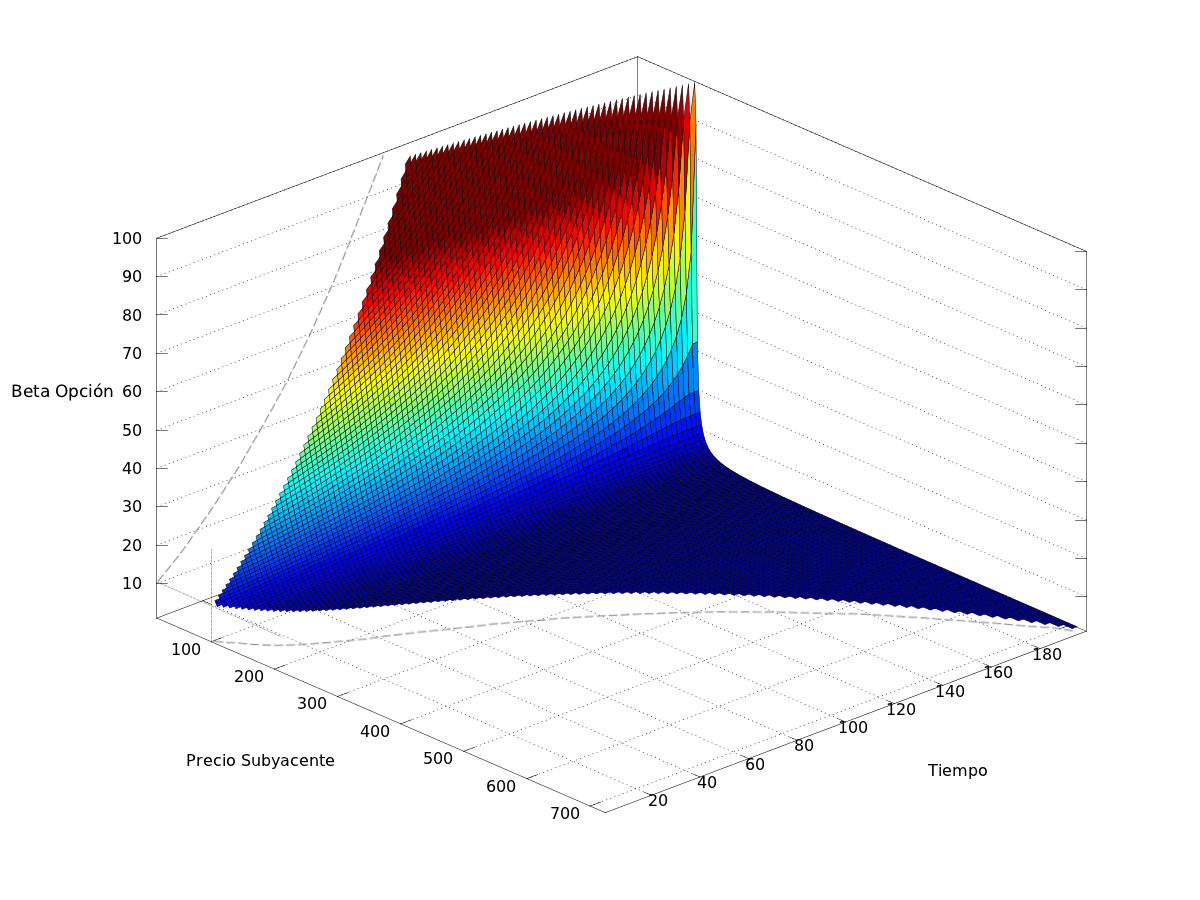
\includegraphics[width=1\textwidth]{Images/beta3d.png}
\caption{Evolución de la $\beta$ de la opción en el árbol binomial}
\label{fig:beta3d}
\end{figure}

Si se evalúa la evolución del \textit{beta} a lo largo del árbol para los mismos precios del subyacente, se puede observar que esta crece a medida que el plazo a la fecha de ejercicio disminuye. Sin embargo, la relación no es lineal. El crecimiento del \textit{beta} es bajo cuando el plazo al vencimiento es alto y crece rápidamente en los últimos periodos. Esta medida de riesgo, en función del plazo al vencimiento evoluciona de forma exponencial decreciente, de forma que se asemeja a una función del tipo $\beta(T-t) \sim a/(T-t)^b$ donde $a$ y $b$ son parámetros a estimar en cada caso. Esta función no tiene por objetivo ser exacta, sino facilitar la comprensión.

En el caso de las opciones \textit{put} o de venta, el comportamiento del \textit{beta} es análogo y a la vez más complejo. Si se descompone el valor de la opción entre el valor que otorga esta como seguro y el tiempo del dinero, se puede ver que ambos factores afectan de forma contraria al precio. Por esta razón, existen casos en donde el \textit{put} puede tener un \textit{beta} menor a la del activo subyacente \cite{optionsmarkets}.


\section{Más \textit{beta}: Casos particulares}

Existen dos casos particulares en donde el \textit{beta} exhibe valores distintos a los explicados anteriormente. 

Primero, en los nodos del último paso del árbol el \textit{beta} de la opción esta indefinida. Esto se debe a que no tiene sentido hablar de CAPM en un punto especifico ya que los rendimientos y por lo tanto el tiempo son cruciales en este modelo. Dada la definición matemática $\beta_f = Cov(r_f; r_M) / \Sigma_M^2$, la rentabilidad del activo es un parámetro tiempo-dependiente, por lo que la beta puntual no se encuentra definida.

Segundo, existe un área triangular en los últimos nodos del árbol cuando la opción se encuentra \textit{out-of-the-money} en donde el \textit{beta} está también indefinida. La figura \ref{fig:betaarbolchico} muestra este comportamiento. La inexistencia de un valor para el \textit{beta} surge del hecho de que no existe ningún camino posible que conduzca a la opción a estar \textit{in-the-money}. Si la opción vale en esos casos por definición cero ($Cov(r_f; r_M)$), la réplica es posible aunque innecesaria, por lo que el \textit{beta} del activo será indefinida. A medida que se incrementa la cantidad de pasos este error tiende a reducirse aunque nunca se elimina por completo en un árbol binomial.

Como se mencionó anteriormente, estos dos problemas tienden a desaparecer a medida que se incrementa la cantidad de pasos que se utiliza en el árbol binomial, por lo que no invalida el modelo. El segundo problema mencionado es sin duda una de las fuentes de error ya que esto no ocurre en modelos en tiempo continuo.





